\documentclass[11pt,letterpaper,final]{report}
\usepackage[utf8]{inputenc}
\usepackage[francais]{babel}
\usepackage[T1]{fontenc}
\usepackage{amsmath}
\usepackage{amsfonts}
\usepackage{amssymb}
\usepackage{graphicx}
\usepackage{lmodern}
\usepackage[left=2.54cm,right=2.54cm,top=2.54cm,bottom=2.54cm]{geometry}
\begin{document}
\chapter{Cross validation entre les différentes plateformes de simulations}
\section{Validation Psim/SPS}
\subsection{DCP/DCN}
Pour commencer, parlons d'éléments simples. On a remarqué que la fonction mean de SPS et de PSIM fonctionne différemment. Voici les résultats obtenu de l'utilisation de la fonction mean sur charge RL alimenté par une tension SINUS de 110V crête à 1KHz.
\begin{figure}[h!]
\centering
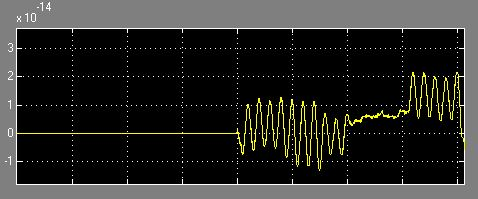
\includegraphics[scale=0.8]{mean_SPS.jpg}
\caption{Réponse de la function Mean sur SPS}
\end{figure}
\begin{figure}[h!]
\centering
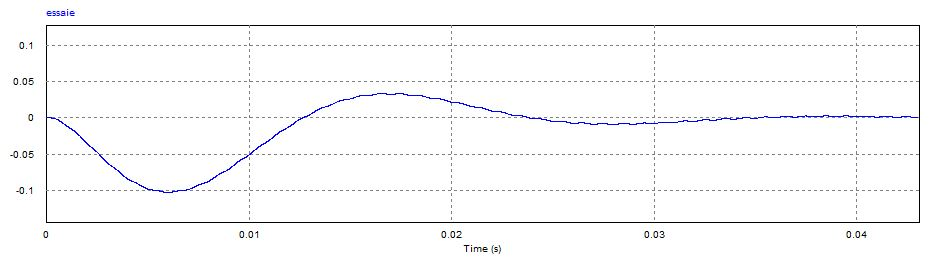
\includegraphics[scale=0.5]{mean_PSIM.jpg}
\caption{Réponse de la function Mean sur PSIM}
\end{figure}

Ces images représentent bien la différence de fonctionnement de ces blocs. On remarque que la fonction mean de SPS a un retard avant qu'il commence à calculer une valeur. PSIM n'a pas cette période d'attente. Par contre, la fonction mean de SPS est plus précise que celle de PSIM qu'on remarque bien  avec la différence de précision des résultats obtenus.
\begin{figure}[h!]
\centering
\includegraphics[scale=0.8]{erreur_PSIM.jpg}
\caption{La différence entre la référence de courant et la valeur obtenu pour PSIM}
\end{figure}

\begin{figure}[h!]
\centering
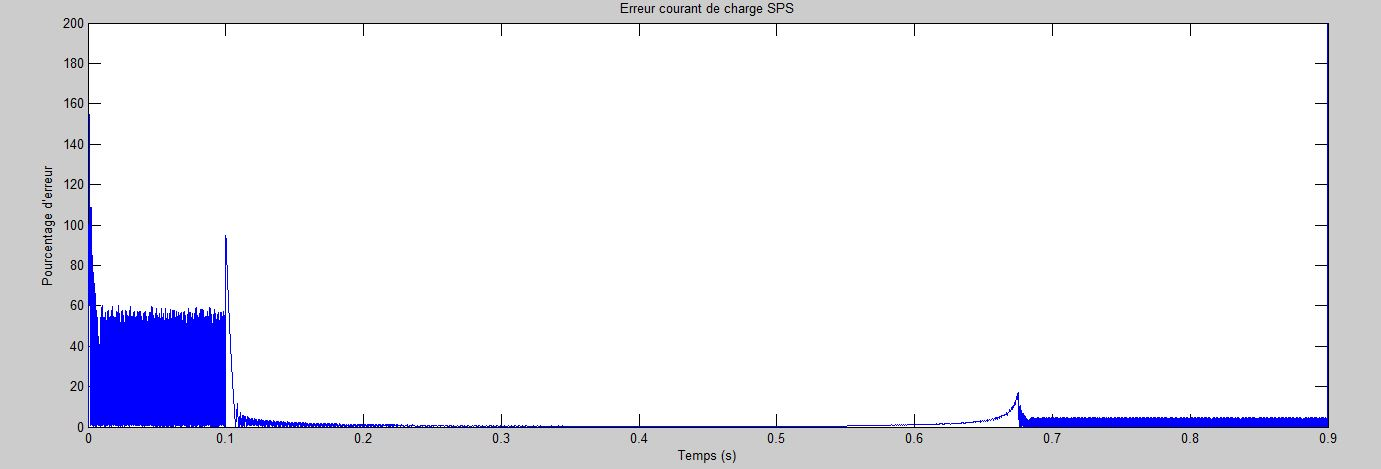
\includegraphics[scale=0.5]{erreur_SPS.jpg}
\caption{La différence entre la référence de courant et la valeur obtenu pour SPS}
\end{figure}

\begin{figure}[h!]
\centering
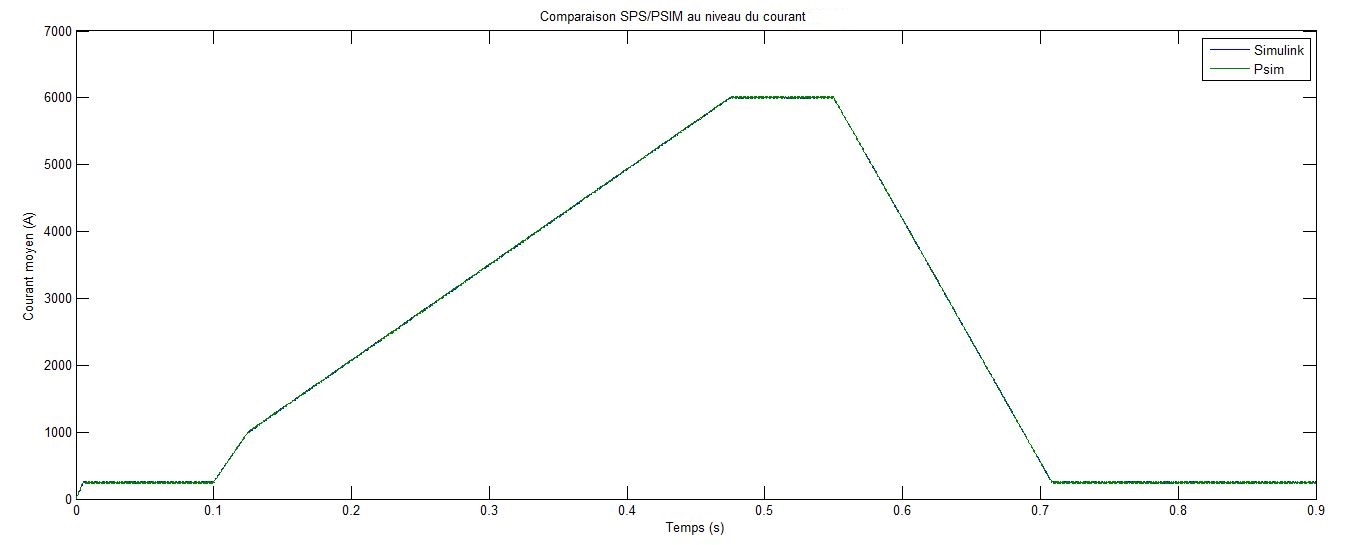
\includegraphics[scale=0.5]{comp_PSIM_SPS.jpg}
\caption{L'erreure entre PSIM et SPS}
\label{comp_PSIM_SPS}
\end{figure}

On remarque bien que les deux simulateurs ne sont pas parfaitement semblables pour l'instant comme le montre la figure~\ref{comp_PSIM_SPS}. Cette différence peut être causé par le filtre de SPS et PSIM qui sont pas le même et à cause que la tension AC au niveau de la charge n'est pas semblable. 

\end{document}